\section{F25 benchmark: reconstruction and extension of Fernandes et al.\ (2025)}
\label{sec:f25_methods}

This section describes the completed classification study. F25-R reconstructs
the ten-class multi-damage benchmark of Fernandes et
al.~\cite{fernandes2025early} with its two original response channels; F25-X
extends it to six vehicle responses and to a CNN with multi-rate pooling. Both
use the same simulated passages, data partition, measurement noise, and
initialization seeds, so their differences are not affected by resampling of
the dataset. F25 is a classification study of ten fixed damage scenarios. It is
independent of the regression campaign described in
Sections~\ref{sec:framework}--\ref{sec:data_processing} and provides none of
its outcomes.

\subsection{Bridge model and damage scenarios}

The bridge is the two-span railway viaduct of the source study: an
Euler--Bernoulli beam with $E=35$~GPa at 15~$^{\circ}$C, $I=0.33$~m$^4$, a mass
of 9,600~kg/m, and 3\% Rayleigh damping, crossed by the five-vehicle train and
layered track of Section~\ref{sec:ttbi}. The source text describes two 20~m
spans, whereas its finite-element grid of 133 elements of 0.30~m corresponds to
a 39.9~m deck with two 19.95~m spans; the latter geometry is reproduced here.
The deck is discretized into 266 elements of 0.15~m. This uniform refinement
keeps every node of the source grid and places the central support, which lies
inside an element of the source grid, on a node. The healthy vertical stiffness
of the central support is $k_v=3.44\times10^{8}$~N/m, and both end bearings are
free to rotate~\cite{fernandes2025early}.

Table~\ref{tab:f25_scenarios} lists the ten scenarios. Scour is represented by a
5\% or 10\% reduction of $k_v$. Bearing damage is represented by a rotational
stiffness of $10^{9}$~N\,m/rad at the entrance bearing. The source models a
crack with the tapered flexural-rigidity law of Sinha et
al.~\cite{sinha2002simplified}, located at the mid-span of the second span, and
reports that crack-depth ratios of 0.10 and 0.05 correspond to $EI$ reductions
of approximately 22\% and 14\% for a 0.30~m element. Here those reductions are
applied uniformly over the same 0.30~m zone, $29.70\le x\le30.00$~m, which
consists of two refined elements. The crack-depth ratios are kept as class
labels; they are not depths calibrated for the uniform surrogate.

\begin{table}[htbp]
\centering
\caption{Damage scenarios of the F25 benchmark~\cite{fernandes2025early}. The
crack label is the source crack-depth ratio; the simulated intervention is the
listed uniform $EI$ reduction. Bearing damage denotes the rotational restraint
of the entrance bearing.}
\label{tab:f25_scenarios}
\small
\begin{tabular}{lrrrc}
\toprule
Scenario & Crack label (\%) & $EI$ reduction (\%) & Scour, $k_v$ reduction (\%) & Bearing damage \\
\midrule
Healthy & 0 & 0 & 0 & -- \\
DC2 & 10 & 22 & 0 & -- \\
DC3 & 0 & 0 & 5 & -- \\
DC4 & 0 & 0 & 0 & yes \\
DC5 & 0 & 0 & 10 & yes \\
DC6 & 10 & 22 & 10 & -- \\
DC7 & 10 & 22 & 0 & yes \\
DC8 & 10 & 22 & 10 & yes \\
DC9 & 10 & 22 & 5 & yes \\
DC10 & 5 & 14 & 5 & yes \\
\bottomrule
\end{tabular}
\end{table}

\subsection{Operational variability and simulated measurements}

Each scenario is simulated for 200 passages, giving 2,000 passages. For each
scenario a Latin hypercube~\cite{mckay1979comparison} of 17 variables is drawn:
the train speed (70--90~km/h), the temperature (3--33~$^{\circ}$C), and, for each
of the five vehicles, the carbody mass (33,000--40,000~kg) and the primary and
secondary suspension stiffnesses (2,640--2,920 and 942--1,042~kN/m per side,
doubled in the planar model). These are the ranges of the source
study~\cite{fernandes2025early}. Temperature modifies the deck modulus as
$E(T)=E_{15}\,[1-0.003\,(T-15)]$. The rail profile is the stored FRA class-4
realization used by Fernandes et al.~\cite{fernandes2024driveby,
fernandes2025early}; it is the same for every passage and scenario and differs
from the generated realization adopted for the regression campaign. Every
passage satisfied the wheel--rail contact admissibility check of the solver.

Following the source, the responses of the leading vehicle are monitored while
its axles cross the bridge, approximately from the entry of the first axle to
the exit of the last one, and are resampled at 100 samples/m. The source reports
a 58.3~m window of 5,830 samples. Its window convention, which uses a 40~m
bridge term, yields 5,831 inclusive samples on the present grid, and the last
sample is discarded. The resulting window is nine samples (0.09~m) longer than
a window computed with the exact 39.9~m deck length.

\subsection{Data partition, measurement noise, and preprocessing}

The passages of each scenario are split into 80 training, 20 validation, and
100 test passages, as in the source. The allocation is a single random
permutation of the local passage indices (PCG64 generator, seed 2025080901),
applied identically to all scenarios and all configurations; the training,
validation, and test sets therefore contain 800, 200, and 1,000 passages. Each
scenario corresponds to one fixed structural configuration, so this split
measures the recognition of known configurations under new operational
conditions, not generalization to unseen damage states.

Measurement noise follows Eq.~(2) of the source~\cite{fernandes2025early}:
\begin{equation}
    x^{\mathrm{noisy}}_i=x_i+0.05\,\sigma(x)\,\epsilon_i,
    \qquad \epsilon_i\sim\mathcal{N}(0,1),
    \label{eq:f25_noise}
\end{equation}
where $\sigma(x)$ is the standard deviation of the clean signal $x$ of one
passage and channel. One noise realization is generated for each scenario,
passage, and channel and is shared by all representations and models. Each
channel is then min--max normalized,
\begin{equation}
    \tilde{x}_i=\frac{x_i-x_{\min}}{x_{\max}-x_{\min}},
\end{equation}
with $x_{\min}$ and $x_{\max}$ computed on the training set only and applied
without clipping to the validation and test sets. RAW inputs keep all 5,830
normalized samples. PAA inputs~\cite{keogh2001dimensionality} replace each
block of ten consecutive samples by its mean, giving 583 values per channel, the
segment length selected in the source study.

\subsection{Response channels}

Six responses of the leading vehicle are considered (Fig.~\ref{fig:model}a):
the vertical accelerations of the carbody (S00), front bogie (S01), and rear
bogie (S02), and the pitch rates of the carbody (S05), front bogie (S06), and
rear bogie (S07). F25-R uses S00 and S01, the carbody and front-bogie sensors of
the source study, each as a single input. F25-X considers all six single
channels and all 15 two-channel combinations. Wheelset accelerations are not
used: in the planar model the wheelsets follow the rail, so their accelerations
are kinematic quantities rather than independent responses
(Section~\ref{sec:response_channels}).

\subsection{CNN architectures}

RAW-CNN and PAA-CNN reproduce the source architecture
(Fig.~\ref{fig:f25_architecture}): one to five valid one-dimensional
convolutions with ReLU activation, each optionally followed by max pooling of
size two, a flatten layer, a dense ReLU layer, and a ten-class output layer.
PAA-MR (PAA with multi-rate pooling) replaces the flatten layer by adaptive
max pooling at resolutions of 1, 2, and 4 bins, inspired by the multi-rate
idea of N-HiTS~\cite{challu2023nhits}, and concatenates the seven pooled values
of each feature map before the dense layer. Flattening already preserves the
position of features along the bridge, so multi-rate pooling is an alternative
aggregation rather than a means of adding positional information. It also
reduces the width of the dense-layer input and the number of parameters, so an
accuracy difference between the arms cannot be attributed to a single
mechanism.

\begin{figure}[htbp]
\centering
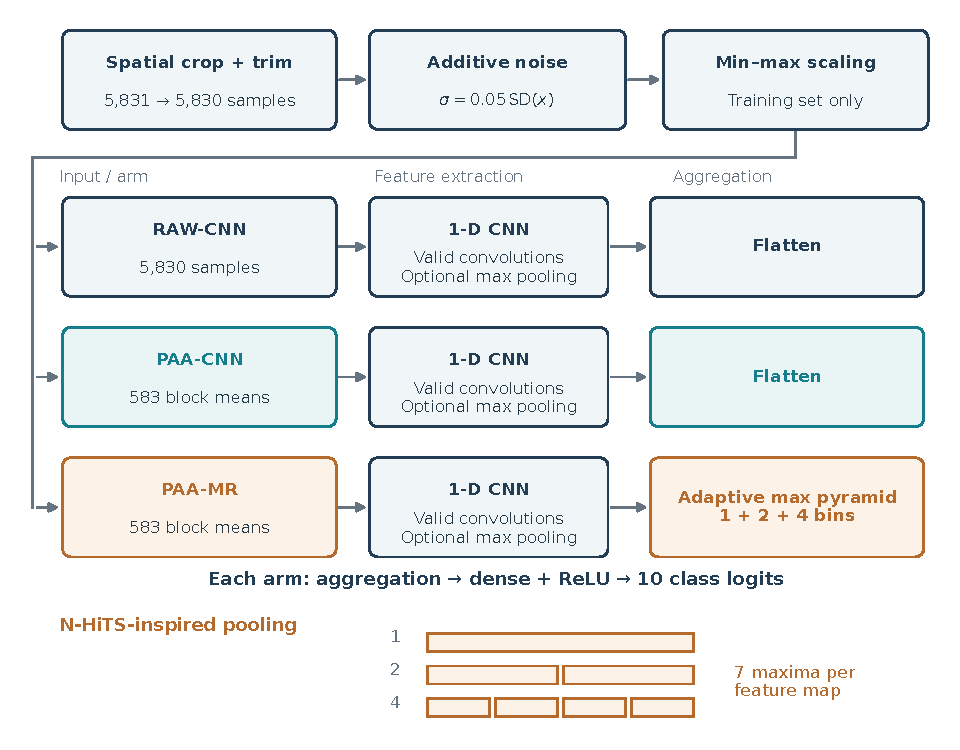
\includegraphics[width=0.92\textwidth]{f25_architecture.pdf}
\caption{Preprocessing and classifier arms of the F25 benchmark. RAW-CNN and
PAA-CNN flatten the last feature maps; PAA-MR replaces flattening with adaptive
max pooling at 1, 2, and 4 bins, giving seven values per feature map. All arms
end in a dense ReLU layer and ten class outputs.}
\label{fig:f25_architecture}
\end{figure}

\subsection{Hyperparameter optimization and training}

Hyperparameters are tuned by Bayesian optimization with the tree-structured
Parzen estimator~\cite{bergstra2011algorithms} implemented in
Optuna~\cite{akiba2019optuna}. As in the source, each optimization comprises
100 proposals, and each proposal is trained five times, here with fixed seeds;
the objective is the mean validation accuracy of the five runs. The search space
is that of the source: one to five convolutional layers, 32--128 filters in
steps of 16, kernel sizes of 2--5, optional max pooling after each layer, 16--64
dense units in steps of 16, batch sizes of 8--48 in steps of 8, and a learning
rate between $10^{-5}$ and $10^{-2}$, sampled on a logarithmic scale.

Networks are trained with the Adam optimizer~\cite{kingma2015adam} and the
cross-entropy loss. The learning rate is halved after 30 epochs without
improvement of the validation loss, down to $10^{-6}$; training stops after 50
epochs without improvement or at 1,000 epochs, and the weights with the lowest
validation loss are restored. These settings follow the source. The test set is
never used for tuning or for checkpoint selection. Each reported configuration
is finally trained with 20 initialization seeds that differ from the five
tuning seeds, and the complete 20-run distribution is reported. The models were
implemented in PyTorch~\cite{paszke2019pytorch} with deterministic GPU
algorithms.

\subsection{Experimental tiers}

F25-R tunes RAW-CNN and PAA-CNN separately for S00 and S01, as in the source.
F25-X comprises three tiers. In the frozen-single tier, the F25-R
hyperparameters tuned for the front bogie (S01) are applied to all six channels;
PAA-MR uses the PAA-CNN vector with only the pooling replaced. In the
tuned-single tier, each of the 18 arm--channel combinations receives its own
100-proposal optimization. In the frozen-pair tier, the frozen vectors are
applied to all 45 arm--pair combinations. The frozen tiers compare channels
under a common architecture, whereas the tuned tier compares them after
channel-specific tuning; a tuned--frozen difference therefore combines the
effect of tuning with the randomness of a finite search. The frozen S01 RAW-CNN
and PAA-CNN configurations repeat the F25-R ones and reproduce their results
exactly, so they are not additional evidence. In total, F25 comprises 22
optimizations and 85 reported configurations, that is, 11,000 tuning runs and
1,700 reported runs.

\subsection{Deviations from the source study}

F25-R is a publication-faithful reconstruction rather than an exact
replication. Table~\ref{tab:f25_deviations} lists the deliberate changes and
the choices that the publication does not report.

\begin{table}[htbp]
\centering
\caption{Differences between F25-R and the source study~\cite{fernandes2025early}.}
\label{tab:f25_deviations}
\small
\begin{tabular}{@{}>{\raggedright\arraybackslash}p{0.22\textwidth}
>{\raggedright\arraybackslash}p{0.33\textwidth}
>{\raggedright\arraybackslash}p{0.37\textwidth}@{}}
\toprule
Item & Source study & F25-R \\
\midrule
Deck mesh & 0.30~m; central support inside an element & 0.15~m uniform refinement; support on a node \\
Crack model & Tapered local $EI$ law~\cite{sinha2002simplified} & Uniform 22\% or 14\% $EI$ reduction over the same 0.30~m zone \\
Software & TensorFlow & PyTorch \\
Data split & Counts reported; allocation not reported & One seeded permutation shared by all scenarios \\
Min--max scaling & Calibration data not reported & Training set only, per channel \\
Learning-rate sampling & Range reported; distribution not reported & Logarithmic \\
Front-bogie finalist & Dense layer of 96 units, outside the reported 16--64 range & Search restricted to the reported range; the published finalists were not retrained \\
Monitoring window & 5,830 samples (58.3~m) & 5,831 inclusive samples, last one discarded \\
\bottomrule
\end{tabular}
\end{table}

\subsection{Performance metrics}

The main metric is the overall accuracy over the 1,000 test passages; with 100
test passages per scenario, it equals the mean recall of the ten scenarios.
Bearing, scour, and crack accuracies are obtained by mapping the predicted
scenario to its coordinates in Table~\ref{tab:f25_scenarios}: bearing damage
(present or absent), scour level (0, 5, or 10\%), and crack label (0, 5, or
10\%). They are projections of the ten-class prediction, not separately
trained classifiers. Confusion matrices are averaged over the 20 runs, with
rows denoting true scenarios. Means, sample standard deviations (SD), medians,
and seed-paired differences describe the variability caused by network
initialization for one fixed data partition; they are not confidence intervals
for other datasets or for field conditions. Because all configurations are
ranked on the same test set, rankings across channels and pairs are
exploratory, and the regression campaign does not use them to select its
response pair.
